%*****************************************
\chapter{Implementation}
\label{ch:implementation}
%*****************************************

%\hint{This chapter should describe the details of the implementation addressing the following questions: \\ \\
%1. What are the design decisions made? \\
%2. What is the environment the approach is developed in? \\
%3. How are components mapped to classes of the source code? \\
%4. How do the components interact with each other?  \\
%5. What are limitations of the implementation? \\ \\
%The section should have a length of about five pages.}

Up to this point, this paper presents discussions on a conceptual level. In contrast, this chapter examines the actual execution of the previously presented experiments.

\section{Representation of the components}
In chapter \ref{ch:design}, an experiment is defined mainly by its architecture, its training parameters, and its pruning setup. Figure \ref{fig:Setup Representation} clarifies where those components can be found in the framework.
Additionally, figure \ref{fig:Dataset Representation} describes which datasets are available and which were preprocessed. The natural language dataset, Reuters-21578, consists of legacy code that was not used in any of the presented experiments. It was implemented during the research phase of this thesis.
\begin{figure}
	\begin{minipage}{0.45\textwidth}
		\centering
		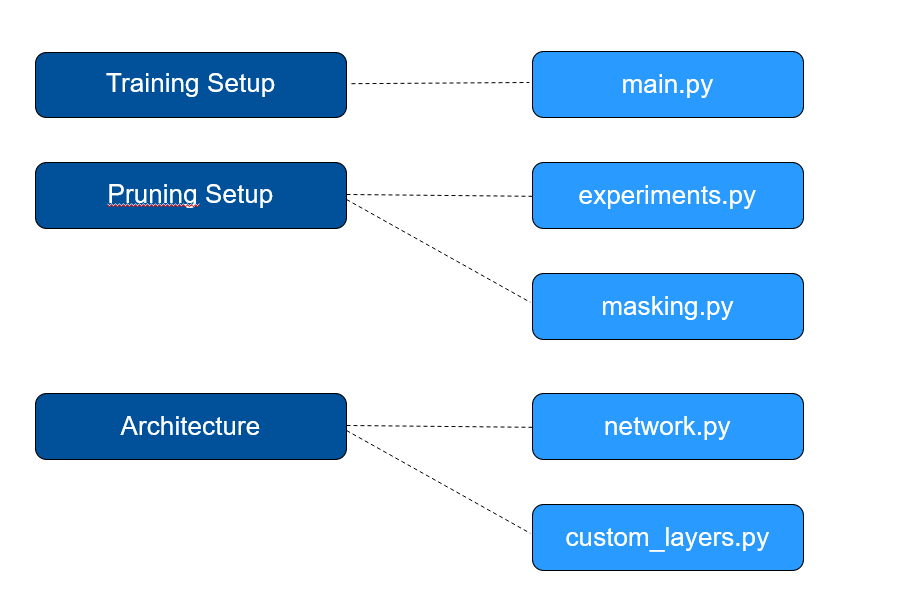
\includegraphics[width=200px]{gfx/chp_5_setups.png}
		\caption{Representation of the main components in the framework}
		\label{fig:Setup Representation}
	\end{minipage}\hfill
	\begin{minipage}{0.45\textwidth}
		\centering
		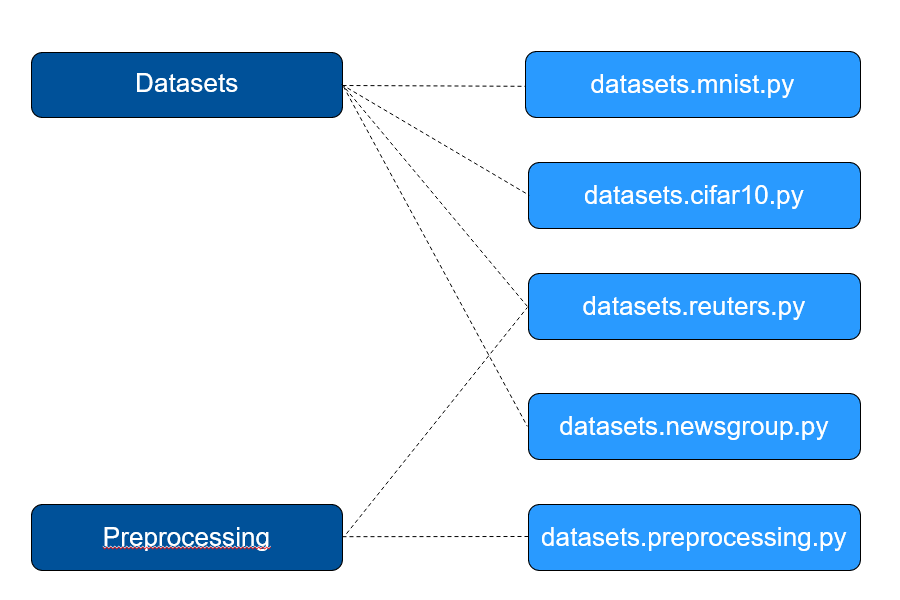
\includegraphics[width=200px]{gfx/chp_5_datasets.png}
		\caption{project architecture}
		\label{fig:Dataset Representation}
	\end{minipage}
\end{figure}
%\begin{figure}[h]
%	\centering
%	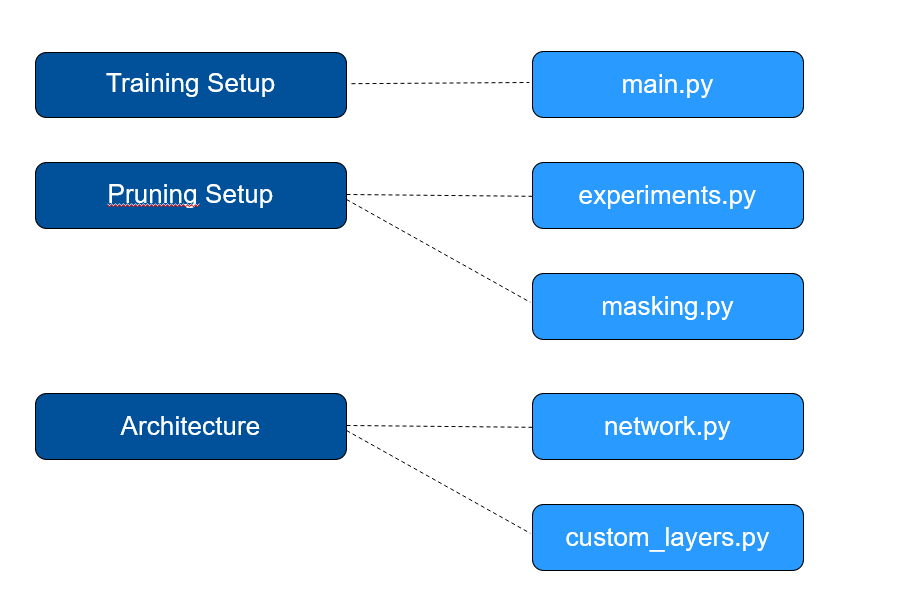
\includegraphics[width=450px]{gfx/chp_5_setups.png}
%	\caption{Representation of the main components in the framework}
%	\label{fig:Setup Representation}
%\end{figure}
%\begin{figure}[h]
%	\centering
%	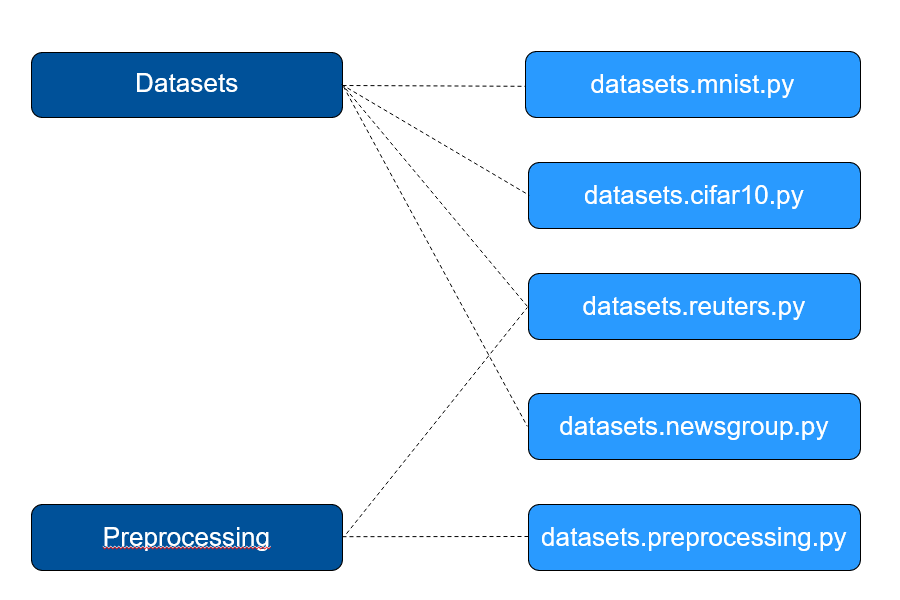
\includegraphics[width=450px]{gfx/chp_5_datasets.png}
%	\caption{project architecture}
%	\label{fig:Dataset Representation}
%\end{figure}

\section{Execution Flow}
The framework differentiates three layers of abstraction. Any single module should only ever use data on the same level of abstraction.
The highest layer defines the training setup, chooses parameters for the remaining layers, collects the resulting training histories, and saves them. Optionally the results can be visualized, either directly or from saved files. 
On the next layer, the framework loads the dataset and instantiates the network wrapper. Afterward, it trains the network while collecting metrics into histories, and prunes it when appropriate.
The lowest layer of the framework forms the interface to the neural network backend. Here, architectures are implements, models are trained models, and weights are masked to model the pruning of connections.
Figure \ref{fig:Example Control Flow} depicts a scheme of the framework during one of the experiments. The highlighted pieces define the execution flow.
\begin{figure}
	\centering
	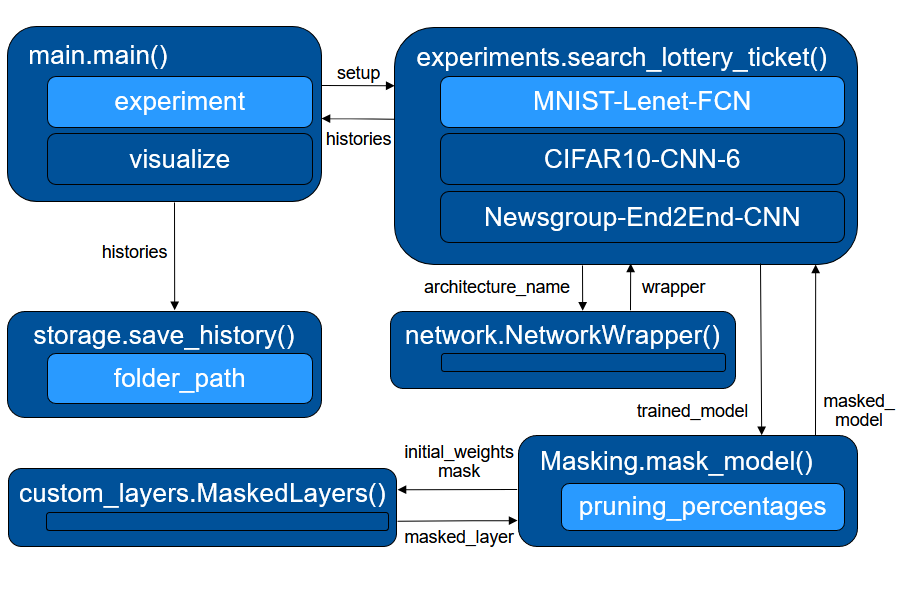
\includegraphics[width=450px]{gfx/chp_5_control_flow.png}
	\caption{Scheme of the framework during an example experiment}
	\label{fig:Example Control Flow}
\end{figure}

\section{Backend}
\subsection{Networks}
Tensorflow 2.0 supplies a functional API capable of implementing all networks described in this thesis and many more. It also brings execution to other devices than the regular CPU core.\cite{Tensorflow} Of particular interest to this work is the speed-up achieved through the usage of GPUs. 
\subsection{Datasets and Preprocessing}
MNIST and CIFAR10 have an interface in Tensorflow 2.0. The corresponding modules of the supplied framework read out these interfaces, bring the data into the expected shape, and then split them canonically into training and test datapoints. 
For 20Newsgroup and Reuters-21578, the backend integrates NLTK, an open-source natural language framework. NLTK also supplies a Word Tokenizer, which splits a raw text into word-like tokens.\cite{NLTK}
\subsection{I/O-Elements}
The supplied framework employs the object-serialization package pickle to save the history of an experiment directly. This type of storage is a solution for internal use only. On their website, the packages authors explicitly warn of untrusted pickle files.

\section{Limitations}
While the code available alongside this thesis is generally capable of unraveling and reproducing any architecture described in the functional API of Tensorflow 2.0, it only supports the masking of the layers described in chapter \ref{ch:design}. 
Additionally, Tensorflow 2.0 itself does not support the pruning of single neural connections because they are bundled together in the tensors used to model layers. As it can only flag whole tensors as non-trainable, a different solution is necessary. While it is less efficient, this thesis' code base resets each pruned weight in a masked layer to zero each time it is called.